\documentclass[twoside]{book}

% Packages required by doxygen
\usepackage{fixltx2e}
\usepackage{calc}
\usepackage{doxygen}
\usepackage[export]{adjustbox} % also loads graphicx
\usepackage{graphicx}
\usepackage[utf8]{inputenc}
\usepackage{makeidx}
\usepackage{multicol}
\usepackage{multirow}
\PassOptionsToPackage{warn}{textcomp}
\usepackage{textcomp}
\usepackage[nointegrals]{wasysym}
\usepackage[table]{xcolor}

% Font selection
\usepackage[T1]{fontenc}
\usepackage[scaled=.90]{helvet}
\usepackage{courier}
\usepackage{amssymb}
\usepackage{sectsty}
\renewcommand{\familydefault}{\sfdefault}
\allsectionsfont{%
  \fontseries{bc}\selectfont%
  \color{darkgray}%
}
\renewcommand{\DoxyLabelFont}{%
  \fontseries{bc}\selectfont%
  \color{darkgray}%
}
\newcommand{\+}{\discretionary{\mbox{\scriptsize$\hookleftarrow$}}{}{}}

% Page & text layout
\usepackage{geometry}
\geometry{%
  a4paper,%
  top=2.5cm,%
  bottom=2.5cm,%
  left=2.5cm,%
  right=2.5cm%
}
\tolerance=750
\hfuzz=15pt
\hbadness=750
\setlength{\emergencystretch}{15pt}
\setlength{\parindent}{0cm}
\setlength{\parskip}{3ex plus 2ex minus 2ex}
\makeatletter
\renewcommand{\paragraph}{%
  \@startsection{paragraph}{4}{0ex}{-1.0ex}{1.0ex}{%
    \normalfont\normalsize\bfseries\SS@parafont%
  }%
}
\renewcommand{\subparagraph}{%
  \@startsection{subparagraph}{5}{0ex}{-1.0ex}{1.0ex}{%
    \normalfont\normalsize\bfseries\SS@subparafont%
  }%
}
\makeatother

% Headers & footers
\usepackage{fancyhdr}
\pagestyle{fancyplain}
\fancyhead[LE]{\fancyplain{}{\bfseries\thepage}}
\fancyhead[CE]{\fancyplain{}{}}
\fancyhead[RE]{\fancyplain{}{\bfseries\leftmark}}
\fancyhead[LO]{\fancyplain{}{\bfseries\rightmark}}
\fancyhead[CO]{\fancyplain{}{}}
\fancyhead[RO]{\fancyplain{}{\bfseries\thepage}}
\fancyfoot[LE]{\fancyplain{}{}}
\fancyfoot[CE]{\fancyplain{}{}}
\fancyfoot[RE]{\fancyplain{}{\bfseries\scriptsize Generated by Doxygen }}
\fancyfoot[LO]{\fancyplain{}{\bfseries\scriptsize Generated by Doxygen }}
\fancyfoot[CO]{\fancyplain{}{}}
\fancyfoot[RO]{\fancyplain{}{}}
\renewcommand{\footrulewidth}{0.4pt}
\renewcommand{\chaptermark}[1]{%
  \markboth{#1}{}%
}
\renewcommand{\sectionmark}[1]{%
  \markright{\thesection\ #1}%
}

% Indices & bibliography
\usepackage{natbib}
\usepackage[titles]{tocloft}
\setcounter{tocdepth}{3}
\setcounter{secnumdepth}{5}
\makeindex

% Hyperlinks (required, but should be loaded last)
\usepackage{ifpdf}
\ifpdf
  \usepackage[pdftex,pagebackref=true]{hyperref}
\else
  \usepackage[ps2pdf,pagebackref=true]{hyperref}
\fi
\hypersetup{%
  colorlinks=true,%
  linkcolor=blue,%
  citecolor=blue,%
  unicode%
}

% Custom commands
\newcommand{\clearemptydoublepage}{%
  \newpage{\pagestyle{empty}\cleardoublepage}%
}

\usepackage{caption}
\captionsetup{labelsep=space,justification=centering,font={bf},singlelinecheck=off,skip=4pt,position=top}

%===== C O N T E N T S =====

\begin{document}

% Titlepage & ToC
\hypersetup{pageanchor=false,
             bookmarksnumbered=true,
             pdfencoding=unicode
            }
\pagenumbering{alph}
\begin{titlepage}
\vspace*{7cm}
\begin{center}%
{\Large My Project }\\
\vspace*{1cm}
{\large Generated by Doxygen 1.8.13}\\
\end{center}
\end{titlepage}
\clearemptydoublepage
\pagenumbering{roman}
\tableofcontents
\clearemptydoublepage
\pagenumbering{arabic}
\hypersetup{pageanchor=true}

%--- Begin generated contents ---
\chapter{My Personal Index Page}
\label{index}\hypertarget{index}{}\hypertarget{index_intro_sec}{}\section{C\+S\+C\+I3081\+W Lab 9 and 10 -\/ dongx462}\label{index_intro_sec}
\hyperlink{classBus}{Bus} simulation. Generate passengers that travel through buses to get from stop to stop. Buses and passengers are on route to their destination. 
\chapter{Class Index}
\section{Class List}
Here are the classes, structs, unions and interfaces with brief descriptions\+:\begin{DoxyCompactList}
\item\contentsline{section}{\hyperlink{classBus}{Bus} \\*The main class for bus }{\pageref{classBus}}{}
\item\contentsline{section}{\hyperlink{classPassenger}{Passenger} \\*The main class for passenger }{\pageref{classPassenger}}{}
\item\contentsline{section}{\hyperlink{classStop}{Stop} \\*The main class for passenger }{\pageref{classStop}}{}
\end{DoxyCompactList}

\chapter{File Index}
\section{File List}
Here is a list of all documented files with brief descriptions\+:\begin{DoxyCompactList}
\item\contentsline{section}{/home/dongx462/\+C\+S\+C\+I3081/repo-\/dongx462/labs/lab09\+\_\+project\+\_\+intro/src/\hyperlink{bus_8cc}{bus.\+cc} }{\pageref{bus_8cc}}{}
\item\contentsline{section}{/home/dongx462/\+C\+S\+C\+I3081/repo-\/dongx462/labs/lab09\+\_\+project\+\_\+intro/src/\hyperlink{bus_8h}{bus.\+h} }{\pageref{bus_8h}}{}
\item\contentsline{section}{/home/dongx462/\+C\+S\+C\+I3081/repo-\/dongx462/labs/lab09\+\_\+project\+\_\+intro/src/\hyperlink{mainpage_8h}{mainpage.\+h} }{\pageref{mainpage_8h}}{}
\item\contentsline{section}{/home/dongx462/\+C\+S\+C\+I3081/repo-\/dongx462/labs/lab09\+\_\+project\+\_\+intro/src/\hyperlink{passenger_8cc}{passenger.\+cc} }{\pageref{passenger_8cc}}{}
\item\contentsline{section}{/home/dongx462/\+C\+S\+C\+I3081/repo-\/dongx462/labs/lab09\+\_\+project\+\_\+intro/src/\hyperlink{passenger_8h}{passenger.\+h} }{\pageref{passenger_8h}}{}
\item\contentsline{section}{/home/dongx462/\+C\+S\+C\+I3081/repo-\/dongx462/labs/lab09\+\_\+project\+\_\+intro/src/\hyperlink{passenger__driver_8cc}{passenger\+\_\+driver.\+cc} }{\pageref{passenger__driver_8cc}}{}
\item\contentsline{section}{/home/dongx462/\+C\+S\+C\+I3081/repo-\/dongx462/labs/lab09\+\_\+project\+\_\+intro/src/\hyperlink{stop_8cc}{stop.\+cc} }{\pageref{stop_8cc}}{}
\item\contentsline{section}{/home/dongx462/\+C\+S\+C\+I3081/repo-\/dongx462/labs/lab09\+\_\+project\+\_\+intro/src/\hyperlink{stop_8h}{stop.\+h} }{\pageref{stop_8h}}{}
\end{DoxyCompactList}

\chapter{Class Documentation}
\hypertarget{classBus}{}\section{Bus Class Reference}
\label{classBus}\index{Bus@{Bus}}


The main class for bus.  




{\ttfamily \#include $<$bus.\+h$>$}



Collaboration diagram for Bus\+:\nopagebreak
\begin{figure}[H]
\begin{center}
\leavevmode
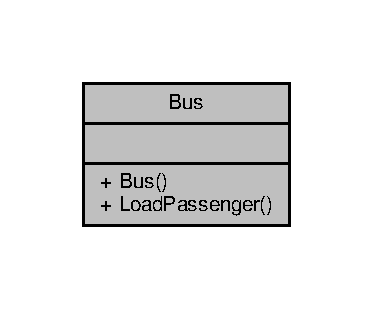
\includegraphics[width=179pt]{classBus__coll__graph}
\end{center}
\end{figure}
\subsection*{Public Member Functions}
\begin{DoxyCompactItemize}
\item 
\hyperlink{classBus_a8a34b953fea6c227c1b2d1102e2ca37b}{Bus} (int capacity=60, double speed=1)
\begin{DoxyCompactList}\small\item\em Constructor for passenger. \end{DoxyCompactList}\item 
bool \hyperlink{classBus_ac3f1c523bc4f97bc8ada8dc488ab3484}{Load\+Passenger} (\hyperlink{classPassenger}{Passenger} $\ast$)
\begin{DoxyCompactList}\small\item\em Loads a passenger onto the buss. \end{DoxyCompactList}\end{DoxyCompactItemize}


\subsection{Detailed Description}
The main class for bus. 

Contains metrics of a bus object 

\subsection{Constructor \& Destructor Documentation}
\mbox{\Hypertarget{classBus_a8a34b953fea6c227c1b2d1102e2ca37b}\label{classBus_a8a34b953fea6c227c1b2d1102e2ca37b}} 
\index{Bus@{Bus}!Bus@{Bus}}
\index{Bus@{Bus}!Bus@{Bus}}
\subsubsection{\texorpdfstring{Bus()}{Bus()}}
{\footnotesize\ttfamily Bus\+::\+Bus (\begin{DoxyParamCaption}\item[{int}]{capacity = {\ttfamily 60},  }\item[{double}]{speed = {\ttfamily 1} }\end{DoxyParamCaption})\hspace{0.3cm}{\ttfamily [explicit]}}



Constructor for passenger. 


\begin{DoxyParams}[1]{Parameters}
\mbox{\tt in}  & {\em capacity,Max} & capacity is 60 by default \\
\hline
\mbox{\tt in}  & {\em speed,Speed} & is 1 by default \\
\hline
\end{DoxyParams}


\subsection{Member Function Documentation}
\mbox{\Hypertarget{classBus_ac3f1c523bc4f97bc8ada8dc488ab3484}\label{classBus_ac3f1c523bc4f97bc8ada8dc488ab3484}} 
\index{Bus@{Bus}!Load\+Passenger@{Load\+Passenger}}
\index{Load\+Passenger@{Load\+Passenger}!Bus@{Bus}}
\subsubsection{\texorpdfstring{Load\+Passenger()}{LoadPassenger()}}
{\footnotesize\ttfamily bool Bus\+::\+Load\+Passenger (\begin{DoxyParamCaption}\item[{\hyperlink{classPassenger}{Passenger} $\ast$}]{new\+\_\+passenger }\end{DoxyParamCaption})}



Loads a passenger onto the buss. 


\begin{DoxyParams}[1]{Parameters}
\mbox{\tt in}  & {\em passenger} & pointer \\
\hline
\end{DoxyParams}


The documentation for this class was generated from the following files\+:\begin{DoxyCompactItemize}
\item 
/home/dongx462/\+C\+S\+C\+I3081/repo-\/dongx462/labs/lab09\+\_\+project\+\_\+intro/src/\hyperlink{bus_8h}{bus.\+h}\item 
/home/dongx462/\+C\+S\+C\+I3081/repo-\/dongx462/labs/lab09\+\_\+project\+\_\+intro/src/\hyperlink{bus_8cc}{bus.\+cc}\end{DoxyCompactItemize}

\hypertarget{classPassenger}{}\section{Passenger Class Reference}
\label{classPassenger}\index{Passenger@{Passenger}}


The main class for passenger.  




{\ttfamily \#include $<$passenger.\+h$>$}



Collaboration diagram for Passenger\+:\nopagebreak
\begin{figure}[H]
\begin{center}
\leavevmode
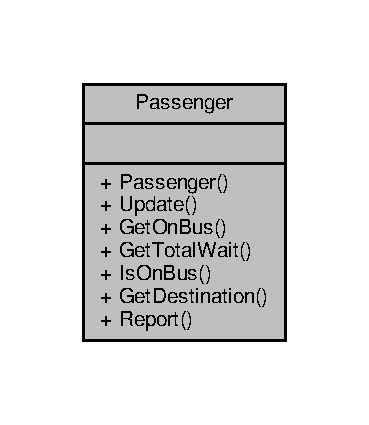
\includegraphics[width=177pt]{classPassenger__coll__graph}
\end{center}
\end{figure}
\subsection*{Public Member Functions}
\begin{DoxyCompactItemize}
\item 
\hyperlink{classPassenger_a5c3addb9a6fd03e5e5642ed844e2702c}{Passenger} (int=-\/1, std\+::string=\char`\"{}Nobody\char`\"{})
\begin{DoxyCompactList}\small\item\em Constructor for passenger. \end{DoxyCompactList}\item 
\mbox{\Hypertarget{classPassenger_a960de3b29fc17a2c2d79c0b79d5cf299}\label{classPassenger_a960de3b29fc17a2c2d79c0b79d5cf299}} 
void \hyperlink{classPassenger_a960de3b29fc17a2c2d79c0b79d5cf299}{Update} ()
\begin{DoxyCompactList}\small\item\em Updates time spent at bus stop. \end{DoxyCompactList}\item 
\mbox{\Hypertarget{classPassenger_ae2ba639cfef39781ac079778578bd9fe}\label{classPassenger_ae2ba639cfef39781ac079778578bd9fe}} 
void \hyperlink{classPassenger_ae2ba639cfef39781ac079778578bd9fe}{Get\+On\+Bus} ()
\begin{DoxyCompactList}\small\item\em Change passenger\textquotesingle{}s status that they\textquotesingle{}re on the bus. \end{DoxyCompactList}\item 
int \hyperlink{classPassenger_a25158560f790ef7ef06d94c414b34f25}{Get\+Total\+Wait} () const
\begin{DoxyCompactList}\small\item\em Returns the total time waiting for bus. \end{DoxyCompactList}\item 
bool \hyperlink{classPassenger_a2acf008ec444afcc859b914ee24add0e}{Is\+On\+Bus} () const
\begin{DoxyCompactList}\small\item\em Returns if passenger is on bus or not. \end{DoxyCompactList}\item 
int \hyperlink{classPassenger_a49db0ee527377aae6077df190a11501c}{Get\+Destination} () const
\begin{DoxyCompactList}\small\item\em Returns destintation ID. \end{DoxyCompactList}\item 
\mbox{\Hypertarget{classPassenger_ac54ce797e412a4895febe10f07dc5df5}\label{classPassenger_ac54ce797e412a4895febe10f07dc5df5}} 
void \hyperlink{classPassenger_ac54ce797e412a4895febe10f07dc5df5}{Report} () const
\begin{DoxyCompactList}\small\item\em Generate report containing passenger details. \end{DoxyCompactList}\end{DoxyCompactItemize}


\subsection{Detailed Description}
The main class for passenger. 

Contains metrics of passengers of the bus system 

\subsection{Constructor \& Destructor Documentation}
\mbox{\Hypertarget{classPassenger_a5c3addb9a6fd03e5e5642ed844e2702c}\label{classPassenger_a5c3addb9a6fd03e5e5642ed844e2702c}} 
\index{Passenger@{Passenger}!Passenger@{Passenger}}
\index{Passenger@{Passenger}!Passenger@{Passenger}}
\subsubsection{\texorpdfstring{Passenger()}{Passenger()}}
{\footnotesize\ttfamily Passenger\+::\+Passenger (\begin{DoxyParamCaption}\item[{int}]{destination\+\_\+stop\+\_\+id = {\ttfamily -\/1},  }\item[{std\+::string}]{name = {\ttfamily \char`\"{}Nobody\char`\"{}} }\end{DoxyParamCaption})\hspace{0.3cm}{\ttfamily [explicit]}}



Constructor for passenger. 


\begin{DoxyParams}[1]{Parameters}
\mbox{\tt in}  & {\em destination\+\_\+stop\+\_\+id,Destination} & \hyperlink{classStop}{Stop} ID \\
\hline
\mbox{\tt in}  & {\em name,Name} & \\
\hline
\end{DoxyParams}


\subsection{Member Function Documentation}
\mbox{\Hypertarget{classPassenger_a49db0ee527377aae6077df190a11501c}\label{classPassenger_a49db0ee527377aae6077df190a11501c}} 
\index{Passenger@{Passenger}!Get\+Destination@{Get\+Destination}}
\index{Get\+Destination@{Get\+Destination}!Passenger@{Passenger}}
\subsubsection{\texorpdfstring{Get\+Destination()}{GetDestination()}}
{\footnotesize\ttfamily int Passenger\+::\+Get\+Destination (\begin{DoxyParamCaption}{ }\end{DoxyParamCaption}) const}



Returns destintation ID. 

\begin{DoxyReturn}{Returns}
Int variable indicating destination 
\end{DoxyReturn}
\mbox{\Hypertarget{classPassenger_a25158560f790ef7ef06d94c414b34f25}\label{classPassenger_a25158560f790ef7ef06d94c414b34f25}} 
\index{Passenger@{Passenger}!Get\+Total\+Wait@{Get\+Total\+Wait}}
\index{Get\+Total\+Wait@{Get\+Total\+Wait}!Passenger@{Passenger}}
\subsubsection{\texorpdfstring{Get\+Total\+Wait()}{GetTotalWait()}}
{\footnotesize\ttfamily int Passenger\+::\+Get\+Total\+Wait (\begin{DoxyParamCaption}{ }\end{DoxyParamCaption}) const}



Returns the total time waiting for bus. 

\begin{DoxyReturn}{Returns}
Int variable indicating total time waiting for bus. 
\end{DoxyReturn}
\mbox{\Hypertarget{classPassenger_a2acf008ec444afcc859b914ee24add0e}\label{classPassenger_a2acf008ec444afcc859b914ee24add0e}} 
\index{Passenger@{Passenger}!Is\+On\+Bus@{Is\+On\+Bus}}
\index{Is\+On\+Bus@{Is\+On\+Bus}!Passenger@{Passenger}}
\subsubsection{\texorpdfstring{Is\+On\+Bus()}{IsOnBus()}}
{\footnotesize\ttfamily bool Passenger\+::\+Is\+On\+Bus (\begin{DoxyParamCaption}{ }\end{DoxyParamCaption}) const}



Returns if passenger is on bus or not. 

\begin{DoxyReturn}{Returns}
F\+A\+L\+SE if not on bus, T\+R\+UE if on bus 
\end{DoxyReturn}


The documentation for this class was generated from the following files\+:\begin{DoxyCompactItemize}
\item 
/home/dongx462/\+C\+S\+C\+I3081/repo-\/dongx462/labs/lab09\+\_\+project\+\_\+intro/src/\hyperlink{passenger_8h}{passenger.\+h}\item 
/home/dongx462/\+C\+S\+C\+I3081/repo-\/dongx462/labs/lab09\+\_\+project\+\_\+intro/src/\hyperlink{passenger_8cc}{passenger.\+cc}\end{DoxyCompactItemize}

\hypertarget{classStop}{}\section{Stop Class Reference}
\label{classStop}\index{Stop@{Stop}}


The main class for passenger.  




{\ttfamily \#include $<$stop.\+h$>$}



Collaboration diagram for Stop\+:\nopagebreak
\begin{figure}[H]
\begin{center}
\leavevmode
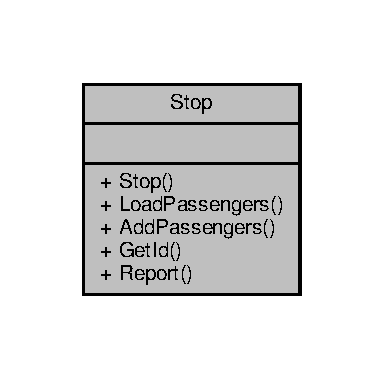
\includegraphics[width=184pt]{classStop__coll__graph}
\end{center}
\end{figure}
\subsection*{Public Member Functions}
\begin{DoxyCompactItemize}
\item 
\hyperlink{classStop_a59d881f072b1cf89512bb15a51ffc773}{Stop} (int, double=44.\+973723, double=-\/93.\+235365)
\begin{DoxyCompactList}\small\item\em Constructor for \hyperlink{classStop}{Stop} class. \end{DoxyCompactList}\item 
\mbox{\Hypertarget{classStop_a5c5c872c082ff6aded344e2cb3e1dc76}\label{classStop_a5c5c872c082ff6aded344e2cb3e1dc76}} 
void \hyperlink{classStop_a5c5c872c082ff6aded344e2cb3e1dc76}{Load\+Passengers} (\hyperlink{classBus}{Bus} $\ast$)
\begin{DoxyCompactList}\small\item\em Removes passengers from stop and onto a bus. \end{DoxyCompactList}\item 
\mbox{\Hypertarget{classStop_a953b0e07fd4a1b7af68e74e5ff7700d0}\label{classStop_a953b0e07fd4a1b7af68e74e5ff7700d0}} 
void \hyperlink{classStop_a953b0e07fd4a1b7af68e74e5ff7700d0}{Add\+Passengers} (\hyperlink{classPassenger}{Passenger} $\ast$)
\begin{DoxyCompactList}\small\item\em Addspassengers to the stop (from the generator) \end{DoxyCompactList}\item 
int \hyperlink{classStop_a2f3b845d5a338f197226c90696314904}{Get\+Id} () const
\begin{DoxyCompactList}\small\item\em Gets \hyperlink{classStop}{Stop} ID. \end{DoxyCompactList}\item 
\mbox{\Hypertarget{classStop_a913202b0c6d4bad1498873251d5d2a2f}\label{classStop_a913202b0c6d4bad1498873251d5d2a2f}} 
void \hyperlink{classStop_a913202b0c6d4bad1498873251d5d2a2f}{Report} () const
\begin{DoxyCompactList}\small\item\em Prints report of stop details and metrics. \end{DoxyCompactList}\end{DoxyCompactItemize}


\subsection{Detailed Description}
The main class for passenger. 

Contains metrics of passengers of the bus system 

\subsection{Constructor \& Destructor Documentation}
\mbox{\Hypertarget{classStop_a59d881f072b1cf89512bb15a51ffc773}\label{classStop_a59d881f072b1cf89512bb15a51ffc773}} 
\index{Stop@{Stop}!Stop@{Stop}}
\index{Stop@{Stop}!Stop@{Stop}}
\subsubsection{\texorpdfstring{Stop()}{Stop()}}
{\footnotesize\ttfamily Stop\+::\+Stop (\begin{DoxyParamCaption}\item[{int}]{id,  }\item[{double}]{longitude = {\ttfamily 44.973723},  }\item[{double}]{latitude = {\ttfamily -\/93.235365} }\end{DoxyParamCaption})\hspace{0.3cm}{\ttfamily [explicit]}}



Constructor for \hyperlink{classStop}{Stop} class. 


\begin{DoxyParams}[1]{Parameters}
\mbox{\tt in}  & {\em stop\+\_\+\+ID,the} & stop ID \\
\hline
\mbox{\tt in}  & {\em longitude\+\_\+,longitude} & is 44.\+973723 by default \\
\hline
\mbox{\tt in}  & {\em latitude\+\_\+,latitude} & is -\/93.\+235365 by default \\
\hline
\end{DoxyParams}


\subsection{Member Function Documentation}
\mbox{\Hypertarget{classStop_a2f3b845d5a338f197226c90696314904}\label{classStop_a2f3b845d5a338f197226c90696314904}} 
\index{Stop@{Stop}!Get\+Id@{Get\+Id}}
\index{Get\+Id@{Get\+Id}!Stop@{Stop}}
\subsubsection{\texorpdfstring{Get\+Id()}{GetId()}}
{\footnotesize\ttfamily int Stop\+::\+Get\+Id (\begin{DoxyParamCaption}{ }\end{DoxyParamCaption}) const}



Gets \hyperlink{classStop}{Stop} ID. 

\begin{DoxyReturn}{Returns}
Returns \hyperlink{classStop}{Stop} ID 
\end{DoxyReturn}


The documentation for this class was generated from the following files\+:\begin{DoxyCompactItemize}
\item 
/home/dongx462/\+C\+S\+C\+I3081/repo-\/dongx462/labs/lab09\+\_\+project\+\_\+intro/src/\hyperlink{stop_8h}{stop.\+h}\item 
/home/dongx462/\+C\+S\+C\+I3081/repo-\/dongx462/labs/lab09\+\_\+project\+\_\+intro/src/\hyperlink{stop_8cc}{stop.\+cc}\end{DoxyCompactItemize}

\chapter{File Documentation}
\hypertarget{bus_8cc}{}\section{/home/dongx462/\+C\+S\+C\+I3081/repo-\/dongx462/labs/lab09\+\_\+project\+\_\+intro/src/bus.cc File Reference}
\label{bus_8cc}\index{/home/dongx462/\+C\+S\+C\+I3081/repo-\/dongx462/labs/lab09\+\_\+project\+\_\+intro/src/bus.\+cc@{/home/dongx462/\+C\+S\+C\+I3081/repo-\/dongx462/labs/lab09\+\_\+project\+\_\+intro/src/bus.\+cc}}
{\ttfamily \#include \char`\"{}bus.\+h\char`\"{}}\newline
Include dependency graph for bus.\+cc\+:\nopagebreak
\begin{figure}[H]
\begin{center}
\leavevmode
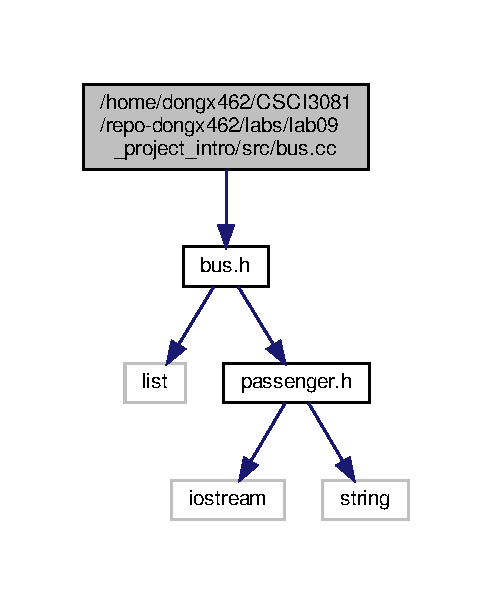
\includegraphics[width=236pt]{bus_8cc__incl}
\end{center}
\end{figure}


\subsection{Detailed Description}
\begin{DoxyCopyright}{Copyright}
2019 3081 Staff, All rights reserved. 
\end{DoxyCopyright}

\hypertarget{bus_8h}{}\section{/home/dongx462/\+C\+S\+C\+I3081/repo-\/dongx462/labs/lab09\+\_\+project\+\_\+intro/src/bus.h File Reference}
\label{bus_8h}\index{/home/dongx462/\+C\+S\+C\+I3081/repo-\/dongx462/labs/lab09\+\_\+project\+\_\+intro/src/bus.\+h@{/home/dongx462/\+C\+S\+C\+I3081/repo-\/dongx462/labs/lab09\+\_\+project\+\_\+intro/src/bus.\+h}}
{\ttfamily \#include $<$list$>$}\newline
{\ttfamily \#include \char`\"{}passenger.\+h\char`\"{}}\newline
Include dependency graph for bus.\+h\+:\nopagebreak
\begin{figure}[H]
\begin{center}
\leavevmode
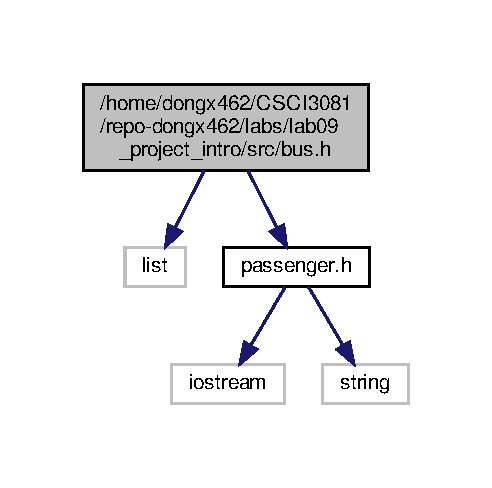
\includegraphics[width=236pt]{bus_8h__incl}
\end{center}
\end{figure}
This graph shows which files directly or indirectly include this file\+:\nopagebreak
\begin{figure}[H]
\begin{center}
\leavevmode
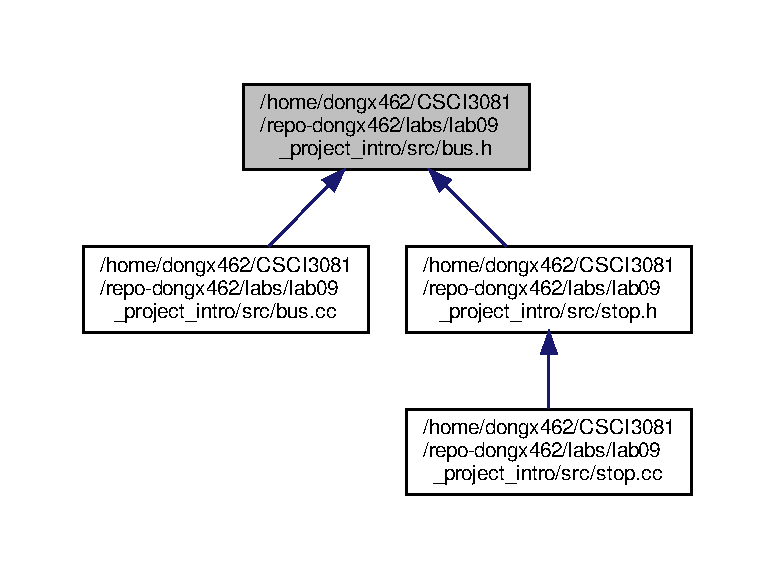
\includegraphics[width=350pt]{bus_8h__dep__incl}
\end{center}
\end{figure}
\subsection*{Classes}
\begin{DoxyCompactItemize}
\item 
class \hyperlink{classBus}{Bus}
\begin{DoxyCompactList}\small\item\em The main class for bus. \end{DoxyCompactList}\end{DoxyCompactItemize}


\subsection{Detailed Description}
\begin{DoxyCopyright}{Copyright}
2019 3081 Staff, All rights reserved. 
\end{DoxyCopyright}

\hypertarget{mainpage_8h}{}\section{/home/dongx462/\+C\+S\+C\+I3081/repo-\/dongx462/labs/lab09\+\_\+project\+\_\+intro/src/mainpage.h File Reference}
\label{mainpage_8h}\index{/home/dongx462/\+C\+S\+C\+I3081/repo-\/dongx462/labs/lab09\+\_\+project\+\_\+intro/src/mainpage.\+h@{/home/dongx462/\+C\+S\+C\+I3081/repo-\/dongx462/labs/lab09\+\_\+project\+\_\+intro/src/mainpage.\+h}}


\subsection{Detailed Description}
\begin{DoxyCopyright}{Copyright}
2019 3081 Staff, All rights reserved. 
\end{DoxyCopyright}

\hypertarget{passenger_8cc}{}\section{/home/dongx462/\+C\+S\+C\+I3081/repo-\/dongx462/labs/lab09\+\_\+project\+\_\+intro/src/passenger.cc File Reference}
\label{passenger_8cc}\index{/home/dongx462/\+C\+S\+C\+I3081/repo-\/dongx462/labs/lab09\+\_\+project\+\_\+intro/src/passenger.\+cc@{/home/dongx462/\+C\+S\+C\+I3081/repo-\/dongx462/labs/lab09\+\_\+project\+\_\+intro/src/passenger.\+cc}}
{\ttfamily \#include $<$iostream$>$}\newline
{\ttfamily \#include $<$string$>$}\newline
{\ttfamily \#include \char`\"{}passenger.\+h\char`\"{}}\newline
Include dependency graph for passenger.\+cc\+:\nopagebreak
\begin{figure}[H]
\begin{center}
\leavevmode
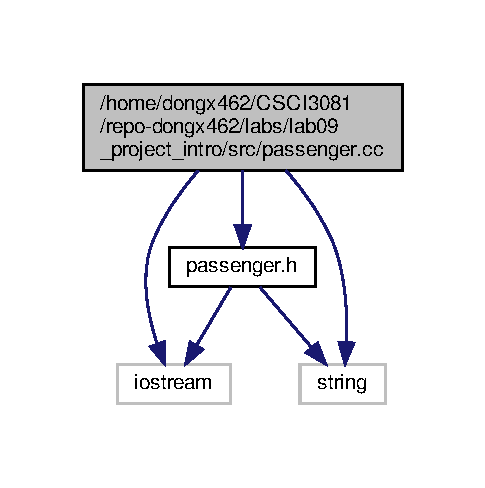
\includegraphics[width=233pt]{passenger_8cc__incl}
\end{center}
\end{figure}


\subsection{Detailed Description}
\begin{DoxyCopyright}{Copyright}
2019 3081 Staff, All rights reserved. 
\end{DoxyCopyright}

\hypertarget{passenger_8h}{}\section{/home/dongx462/\+C\+S\+C\+I3081/repo-\/dongx462/labs/lab09\+\_\+project\+\_\+intro/src/passenger.h File Reference}
\label{passenger_8h}\index{/home/dongx462/\+C\+S\+C\+I3081/repo-\/dongx462/labs/lab09\+\_\+project\+\_\+intro/src/passenger.\+h@{/home/dongx462/\+C\+S\+C\+I3081/repo-\/dongx462/labs/lab09\+\_\+project\+\_\+intro/src/passenger.\+h}}
{\ttfamily \#include $<$iostream$>$}\newline
{\ttfamily \#include $<$string$>$}\newline
Include dependency graph for passenger.\+h\+:\nopagebreak
\begin{figure}[H]
\begin{center}
\leavevmode
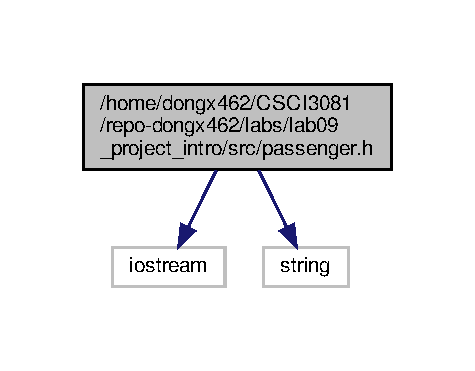
\includegraphics[width=228pt]{passenger_8h__incl}
\end{center}
\end{figure}
This graph shows which files directly or indirectly include this file\+:\nopagebreak
\begin{figure}[H]
\begin{center}
\leavevmode
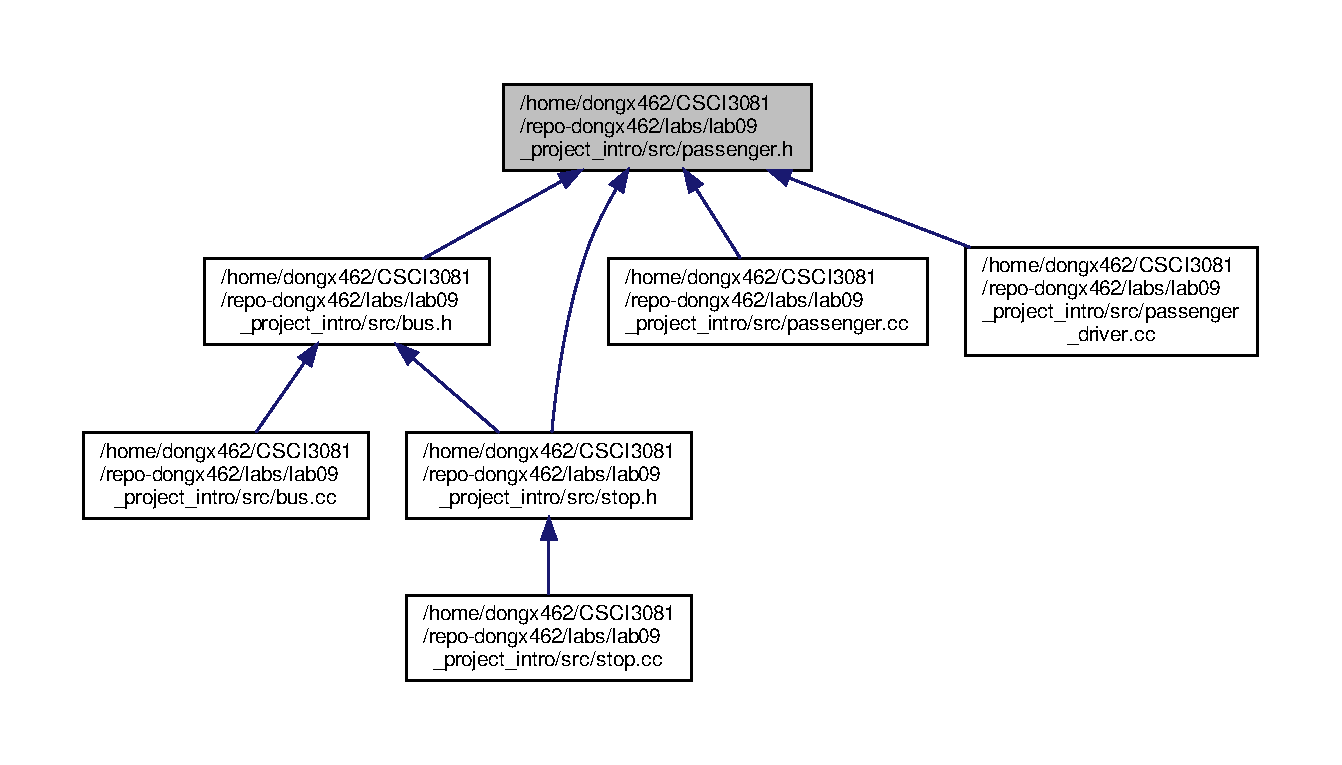
\includegraphics[width=350pt]{passenger_8h__dep__incl}
\end{center}
\end{figure}
\subsection*{Classes}
\begin{DoxyCompactItemize}
\item 
class \hyperlink{classPassenger}{Passenger}
\begin{DoxyCompactList}\small\item\em The main class for passenger. \end{DoxyCompactList}\end{DoxyCompactItemize}


\subsection{Detailed Description}
\begin{DoxyCopyright}{Copyright}
2019 3081 Staff, All rights reserved. 
\end{DoxyCopyright}

\hypertarget{passenger__driver_8cc}{}\section{/home/dongx462/\+C\+S\+C\+I3081/repo-\/dongx462/labs/lab09\+\_\+project\+\_\+intro/src/passenger\+\_\+driver.cc File Reference}
\label{passenger__driver_8cc}\index{/home/dongx462/\+C\+S\+C\+I3081/repo-\/dongx462/labs/lab09\+\_\+project\+\_\+intro/src/passenger\+\_\+driver.\+cc@{/home/dongx462/\+C\+S\+C\+I3081/repo-\/dongx462/labs/lab09\+\_\+project\+\_\+intro/src/passenger\+\_\+driver.\+cc}}
{\ttfamily \#include $<$iostream$>$}\newline
{\ttfamily \#include $<$vector$>$}\newline
{\ttfamily \#include \char`\"{}passenger.\+h\char`\"{}}\newline
Include dependency graph for passenger\+\_\+driver.\+cc\+:\nopagebreak
\begin{figure}[H]
\begin{center}
\leavevmode
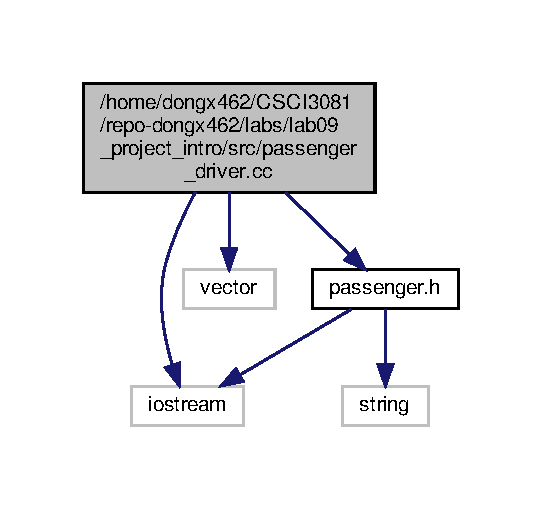
\includegraphics[width=260pt]{passenger__driver_8cc__incl}
\end{center}
\end{figure}
\subsection*{Functions}
\begin{DoxyCompactItemize}
\item 
\mbox{\Hypertarget{passenger__driver_8cc_ae66f6b31b5ad750f1fe042a706a4e3d4}\label{passenger__driver_8cc_ae66f6b31b5ad750f1fe042a706a4e3d4}} 
int {\bfseries main} ()
\end{DoxyCompactItemize}


\subsection{Detailed Description}
\begin{DoxyCopyright}{Copyright}
2019 3081 Staff, All rights reserved. 
\end{DoxyCopyright}

\hypertarget{stop_8cc}{}\section{/home/dongx462/\+C\+S\+C\+I3081/repo-\/dongx462/labs/lab09\+\_\+project\+\_\+intro/src/stop.cc File Reference}
\label{stop_8cc}\index{/home/dongx462/\+C\+S\+C\+I3081/repo-\/dongx462/labs/lab09\+\_\+project\+\_\+intro/src/stop.\+cc@{/home/dongx462/\+C\+S\+C\+I3081/repo-\/dongx462/labs/lab09\+\_\+project\+\_\+intro/src/stop.\+cc}}
{\ttfamily \#include $<$iostream$>$}\newline
{\ttfamily \#include $<$vector$>$}\newline
{\ttfamily \#include $<$list$>$}\newline
{\ttfamily \#include \char`\"{}stop.\+h\char`\"{}}\newline
Include dependency graph for stop.\+cc\+:\nopagebreak
\begin{figure}[H]
\begin{center}
\leavevmode
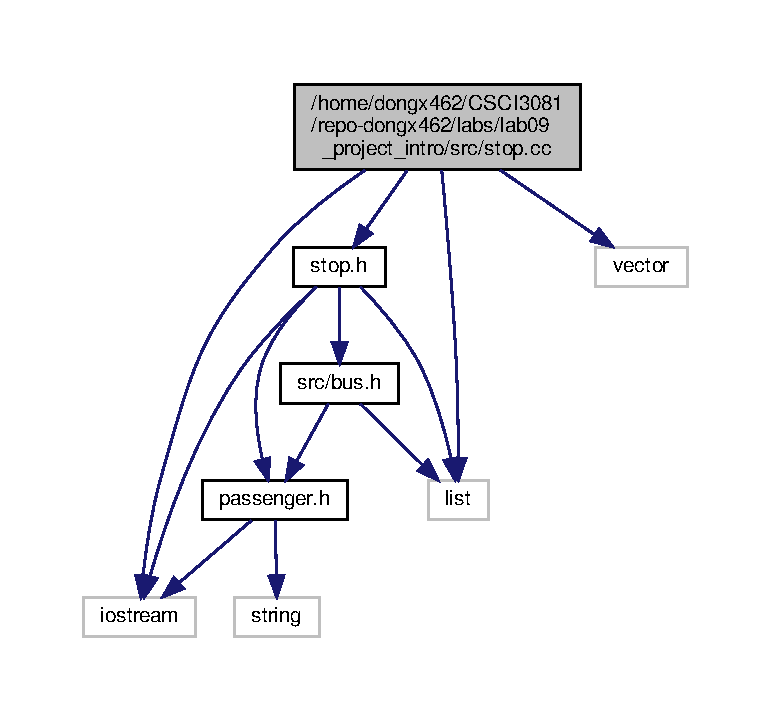
\includegraphics[width=350pt]{stop_8cc__incl}
\end{center}
\end{figure}


\subsection{Detailed Description}
\begin{DoxyCopyright}{Copyright}
2019 3081 Staff, All rights reserved. 
\end{DoxyCopyright}

\hypertarget{stop_8h}{}\section{/home/dongx462/\+C\+S\+C\+I3081/repo-\/dongx462/labs/lab09\+\_\+project\+\_\+intro/src/stop.h File Reference}
\label{stop_8h}\index{/home/dongx462/\+C\+S\+C\+I3081/repo-\/dongx462/labs/lab09\+\_\+project\+\_\+intro/src/stop.\+h@{/home/dongx462/\+C\+S\+C\+I3081/repo-\/dongx462/labs/lab09\+\_\+project\+\_\+intro/src/stop.\+h}}
{\ttfamily \#include $<$list$>$}\newline
{\ttfamily \#include $<$iostream$>$}\newline
{\ttfamily \#include \char`\"{}src/bus.\+h\char`\"{}}\newline
{\ttfamily \#include \char`\"{}src/passenger.\+h\char`\"{}}\newline
Include dependency graph for stop.\+h\+:\nopagebreak
\begin{figure}[H]
\begin{center}
\leavevmode
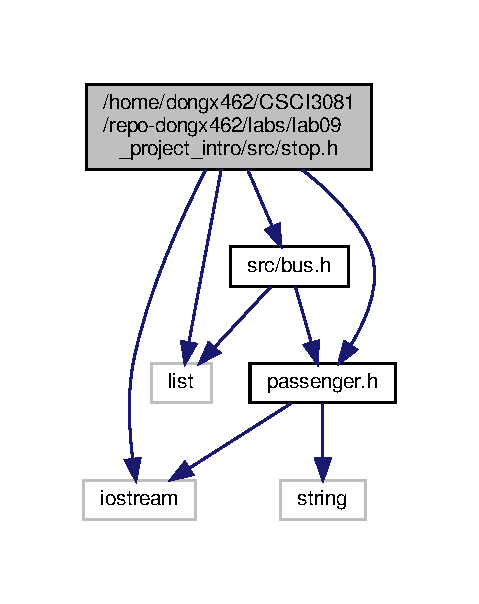
\includegraphics[width=230pt]{stop_8h__incl}
\end{center}
\end{figure}
This graph shows which files directly or indirectly include this file\+:\nopagebreak
\begin{figure}[H]
\begin{center}
\leavevmode
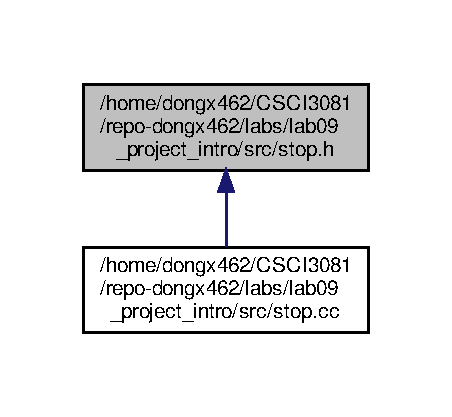
\includegraphics[width=217pt]{stop_8h__dep__incl}
\end{center}
\end{figure}
\subsection*{Classes}
\begin{DoxyCompactItemize}
\item 
class \hyperlink{classStop}{Stop}
\begin{DoxyCompactList}\small\item\em The main class for passenger. \end{DoxyCompactList}\end{DoxyCompactItemize}


\subsection{Detailed Description}
\begin{DoxyCopyright}{Copyright}
2019 3081 Staff, All rights reserved. 
\end{DoxyCopyright}

%--- End generated contents ---

% Index
\backmatter
\newpage
\phantomsection
\clearemptydoublepage
\addcontentsline{toc}{chapter}{Index}
\printindex

\end{document}
